% !TeX root = Stageportfolio.tex



\begin{landscape}
	\section{Lesvoorbereidingen en bijhorende media}
	\subsection{Lessen aan KULAK}
	De bijlagen per lesblok (e.g. bordschema, uitgeschreven oplossingen \ldots) zijn na elk lesblok terug te vinden. De oefeningenlijst wordt bij het eerste lesblok toegevoegd, maar wordt bij ieder lesblok gebruikt.
	\subsubsection{Les 1-3}
	\begin{tabularx}{1.56\textwidth}{|p{0.35\textwidth}|X|}\hline
		\textbf{Administratieve gegevens}\newline\newline
		Kevin Truyaert\newline\newline
		Universiteit\newline
		Handelsingenieur, 2de fase\newline
		\underline{ECTS-fiche}: De inhoud is terug te vinden op de ECTS fiche: \href{https://onderwijsaanbod.kuleuven.be/syllabi/n/D0W55AN.htm}{https://onderwijsaanbod. kuleuven.be /syllabi/n/D0W55AN.htm} \newline
		\underline{Lesonderwerp}: `Oefenzitting elektromagnetisme: wat zijn de relaties tussen de elektrische kracht, de  elektrische potentiaal, de elektrische flux en de elektrische capaciteit' & \textbf{Doelstellingen}\newline\vspace{0.5cm}
		\underline{Punt op de ECTS-fiche}
		\vspace{-0.5cm}\newline  - Elektriciteit: elektrische lading, elektrisch veld (wetten van Coulomb en Gauss), elektrische flux, elektrische potentiaal, energie in een elektrisch veld \newline
		\underline{Lesdoelen}\newline
		\vspace{-0.75cm}
		\begin{enumerate}[itemsep=0.08\baselineskip]
			\item De studenten kunnen via de wet van Coulomb de elektrostatische kracht tussen ladingen berekenen.
			\item De studenten kunnen de relatie tussen de elektrostatische kracht, het elektrisch veld en een lading toepassen in een probleem.
			\item De studenten kunnen de elektrostatische kracht binnen de tweede wet van Newton herkennen.
			\item De studenten kunnen een Gaussoppervlak in een situatie opstellen.
			\item De studenten zijn in staat om de elektrische flux te bepalen met gebruik van een Gaussoppervlak.
			\item De studenten kunnen het elektrisch veld en de elektrische flux  in functie van de afstand  van een boloppervlak afleiden.
			\item De studenten kunnen het elektrisch veld en de elektrische flux  in functie van de afstand van een opgevulde, geleidende bol afleiden.
			\item De studenten kunnen de gelijkenissen en de verschillen van het elektrisch veld en de elektrische flux in functie van de afstand van een boloppervlak en van een opgevulde, geleidende bol bespreken.
		    \item De studenten kunnen in groep over de oefening discussiëren en samen oplossingsgericht werken.
		\end{enumerate} \\\hline
	\end{tabularx}


	\begin{tabularx}{1.56\textwidth}{|p{0.55\textwidth}|X|}
		\hline
		\multirow{2}{0.55\textwidth}{\textbf{Beginsituatie}\newline De studenten hebben de theorie rond de  begrippen van `Elektrisch veld', `Elektrische potentiaal', `Elektrische flux' en de wet van Coulomb in de week van 12-15 november gezien, twee weken voor de oefenzitting. Hierdoor zullen ze al tijd gehad hebben om de theorie te bekijken, wat aangemoedigd wordt door het maken van een voorbereidende opdracht die ik de week voor de oefenzitting op Toledo plaats.\newline\newline De minderheid van de studenten heeft  interesse bij mechanica, het eerste deel van de cursus, getoond. Het gedeelte over elektromagnetisme ervaren ze meestal interessanter. Er zijn 28 studenten die deze sessie volgen, maar gemiddeld gezien zijn er 25 studenten aanwezig geweest bij de voorbije lessen.\newline\newline Het lokaal kan 30 studenten plaatsen. Ik splits de groep in zeven tafels van vier personen. Er is een dubbel krijtbord ter beschikking en de mogelijkheid tot projectie. Wanneer er geprojecteerd wordt, hangt het projectiescherm grotendeels over beide borden.  }& \textbf{Acties}\newline  - Om de studenten te stimuleren om zelf aan de slag te gaan, wil ik hen in \GreenHighlight{groepjes van vier studenten}{5cm} aan de slag zetten. Hierdoor kan ik gerichtere feedback geven, aangezien de studenten onderling elkaar kunnen aanzetten tot het vinden van oplossingen. \PinkHighlight{Naast de ondersteunende rol, kan ik ook interacties tussen de}{12cm}\PinkHighlight{studenten onderling volgen}{5cm} en inspringen waar nodig: ofwel bij het maken van een fout, of wanneer ik hun uiteenzetting zeer goed vind en er nog dieper op in wil gaan. Dit wil ik steeds vanuit het onderwijsleergesprek proberen te realiseren.  \newline\newline
		- Bij het begin van de les overloop ik nog even de theorie rond de elektrische grootheden en hun onderlinge relaties. Dit zet ik op één van de twee krijtborden en laat ik gedurende de hele les staan. Zo kunnen de studenten steeds makkelijk teruggrijpen naar de theorie. \newline\newline
		- Ik werk niet met projectie, maar noteer alles op het bord, omdat het projectiescherm voor zo goed als beide borden hangt. Hierdoor houd ik een tempo aan waarop de studenten makkelijker kunnen volgen, doordat ik alles zelf ook neerschrijf.  
		
		\\ \cline{2-2}
		  & \textbf{Bronnen}\begin{itemize}
		  	\item Dudal, D., Temmerman, E., Truyaert, K., Heymans, S. (2019). Slides conceptuele natuurkunde
		  	\item Dudal, D., Temmerman, E., Truyaert, K., Heymans, S. (2019). Oefeningenbundel conceptuele natuurkunde
		  	\item Giancoli, D. C. (2008). Physics for scientists and engineers. Pearson Education International.
		  \end{itemize}\\ \hline
	\end{tabularx}


\newpage
	
	\begin{tabularx}{1.56\textwidth}{|p{1.5cm}|p{6cm}|X|p{4cm}|}
		\hline
		\textbf{Nr. lesdoel } & \textbf{Inhoud (timing)}  & \textbf{Organisatie } & \textbf{Media } \\ \hline
		&\underline{Herhaling theorie (15 minuten)}\newline
		De algemene student heeft op dit moment weinig voeling met de te bespreken leerstof, want het is de eerste oefenzitting over dit onderwerp. Dit heb ik zowel de voorbije jaren tijdens mijn oefenzittingen gemerkt als bij de geobserveerde theorielessen. Daarom breng ik de theorie waarop de studenten oefeningen zullen maken nog eens zelf aan bord. Deze behandelt vijf topics: lading, elektrisch veld, elektrische kracht, flux en de elektrische wet van Gauss. Vooral deze laatste vormt een struikelblok voor de studenten. Het is mijn bedoeling om die op verschillende manieren nog eens uitgelegd te hebben.
		&  \underline{Doceren}\newline 
		Ik bouw de te gebruiken theorie op door te starten vanuit de eigenschappen van een lading, dat die een elektrisch veld genereren en dat een elektrisch veld op een andere lading inwerkt door middel van de elektrische kracht. Daarna herhaal ik nog kort eens wat elektrische flux is, om dat tot het grootste probleempunt te komen: de elektrische wet van Gauss.\newline
		Ik wil vooral heel hard benadrukken wat deze wet zegt, door de aparte onderdelen uit te leggen en conceptueel voor te stellen. Ik doe dit vanuit verschillende insteken om zoveel mogelijk studenten mee te hebben. 
		\newline 
		Hierna noteer ik de oefeningen op bord die gemaakt kunnen worden. Dit zijn oefeningen 51 t.e.m. 55, 57 en 56, in die volgorde. Ik verwacht dat deze oefeningen door de betere studenten allemaal gemaakt kunnen worden. Ik verwacht dat de meesten zullen vast komen te zitten bij oefening 54 en 55. Deze gaan namelijk over de elektrische wet van Gauss. Oefeningen 57 en 56 kunnen tijdens de volgende les eventueel ook nog aan bod komen. 
		& Krijtbord (Bordschema, zie bijlage)
		\\ \hline
	\end{tabularx}

\begin{tabularx}{1.56\textwidth}{|p{1.5cm}|p{6cm}|X|p{4cm}|}
	\hline
	\textbf{Nr. lesdoel } & \textbf{Inhoud (timing)}  & \textbf{Organisatie } & \textbf{Media } \\ \hline
	1\newline 2\newline 3\newline 4\newline 5\newline 6\newline 9	&\underline{Oefeningen 51-54 (1 uur)}\newline
	Tijdens deze lesfase maken de studenten oefeningen. Studenten moeten de geziene theorie kunnen omzetten in het toepassen van oefeningen. Introductie oefeningen kunnen moeilijker gelinkt worden met fysische concepten die in het dagelijkse leven aanwezig zijn.  Daarom zijn deze oefeningen heel algemeen.\newline De kern van deze lesfase is om de studenten  inzichten met betrekking tot, het kunnen rekenen met en het kunnen interpreteren van  elektrische velden te laten verwerven.

	&  \underline{Check-in duo / check-in quatro}\newline 
	De studenten maken oefeningen door eerst zelf kort na te denken over hoe ze de oefening kunnen aanpakken. Daarna overleggen ze per twee of per vier (hun keuze) hoe ze de oefening tot een goed eind kunnen brengen.\newline	Tijdens de lesfase loop ik rond en bezoek ik alle zeven tafels van vier personen. Ik stel actief vragen aan de studenten, zeker wanneer ik problemen denk waar te nemen. Tegelijkertijd help ik studenten die actief vragen stellen door middel van een onderwijsleergesprek. \newline
	Ik verwacht dat oefeningen 51 tot en met 53 zeker gemaakt worden en dat iedereen minstens aan oefening 54 begonnen is. Bij de eerste drie oefeningen verwacht ik niet dat ik klassikaal zal moeten tussenkomen.  
	& De studenten gebruiken hun oefeningenbundel en lossen oefeningen op cursusbladen op.
	\\ \hline
\end{tabularx}





\begin{tabularx}{1.56\textwidth}{|p{1.5cm}|p{6cm}|X|p{4cm}|}
	\hline
	\textbf{Nr. lesdoel } & \textbf{Inhoud (timing)}  & \textbf{Organisatie } & \textbf{Media } \\ \hline
		&\underline{Pauze}\newline
	
	
	&    De studenten krijgen 15 minuten pauze en mogen het lokaal verlaten. Op deze manier kunnen ze het laatste uur weer met volle aandacht werken. Dit is nodig aangezien ik wel grotere problemen bij oefeningen 54 en 55 voorzie.\newline
	Wanneer de eerste studenten het lokaal terug binnen sijpelen, sla ik een praatje met hen, waarbij ik niet over de leerstof begin. 
	& 
	\\ \hline
\end{tabularx}



\begin{tabularx}{1.56\textwidth}{|p{1.5cm}|p{6cm}|X|p{4cm}|}
	\hline
	\textbf{Nr. lesdoel } & \textbf{Inhoud (timing)}  & \textbf{Organisatie } & \textbf{Media } \\ \hline
	4\newline 5\newline 6\newline 7 \newline 8 \newline 9	&\underline{Oefeningen 54-55 (40 minuten)}\newline
	Tijdens deze lesfase maken de studenten oefeningen. Studenten moeten de geziene theorie kunnen omzetten in het toepassen van oefeningen. Deze oefeningen handelen over de elektrische wet van Gauss, wat een handige tool is om het elektrisch veld van bepaalde ladingsverdelingen te kunnen berekenen. Ik leg hen uit dat dit handig kan zijn bij het berekenen van elektrische velden van ladingsverdelingen met sferische symmetrieën, of bij het bepalen van de sterkte van de aanwezige ladingen bij het opmeten van het elektrisch veld.  \newline De kern van deze lesfase is om de studenten inzichten tot de elektrische wet van Gauss te laten verwerven. Het is belangrijk dat ze iedere component kunnen verklaren en dat ze er mee kunnen rekenen.
	
	&  \underline{Check-in duo / check-in quatro}\newline 
	De studenten maken oefeningen door eerst zelf kort na te denken over hoe ze de oefening kunnen aanpakken. Daarna overleggen ze per twee of per vier (hun keuze) hoe ze de oefening tot een goed eind kunnen brengen.\newline	Tijdens de lesfase loop ik rond en bezoek ik alle zeven tafels van vier personen. Ik stel actief vragen aan de studenten, zeker wanneer ik problemen denk waar te nemen. Tegelijkertijd help ik studenten die actief vragen stellen door middel van een onderwijsleergesprek. \newline
	Ik verwacht dat ik zeker een klassikaal moment zal moeten inleggen bij oefeningen 54 en 55. Bij oefening 54 zal ik dit relatief snel doen en zal ik hoogstens éénmaal bij iedere groep langs geweest zijn. Hierna beschrijf ik oefening 54 aan het bord waarbij ik de nadruk leg op de interpretatie van de wet van Gauss in dit geval. Ik wil een duidelijk onderscheid maken tussen de componenten die steeds hetzelfde blijven (het sferisch Gaussoppervlak keert steeds in dezelfde vorm terug, ongeacht de situatie)  en de componenten die afhankelijk van de situatie zijn (de ladingsverdeling). Ik behandel de twee subvragen apart en vraag na iedere subvraag of de studenten vragen hebben. \newline
	Wanneer dit op het bord staat, leid ik oefening 55 in, door de analogie met oefening 54 te maken en te zeggen hoe de situatie veranderd is. Hiermee gaan ze opnieuw zelf aan de slag. Ik zal deze oefening opnieuw klassikaal bespreken. Hierna vraag ik aan de studenten om mij het verschil tussen het elektrisch veld en de flux van een boloppervlak en een bol met constante ladingsverdeling.
	& De studenten gebruiken hun oefeningenbundel en lossen oefeningen op cursusbladen op. Ik gebruik het tweede bord om oefeningen 54 en 55 op uit te werken. Na oefening 54 behandeld te hebben, vat ik de oplossing samen op het linkerbord om die met de oplossing van oefening 55 te kunnen vergelijken.
	\\ \hline
\end{tabularx}



\begin{tabularx}{1.56\textwidth}{|p{1.5cm}|p{6cm}|X|p{4cm}|}
	\hline
	\textbf{Nr. lesdoel } & \textbf{Inhoud (timing)}  & \textbf{Organisatie } & \textbf{Media } \\ \hline
	1\newline 2\newline 3\newline 9	&\underline{Oefeningen 57 (15 minuten)}\newline
	Tijdens deze lesfase maken de studenten oefeningen. Studenten moeten de geziene theorie kunnen omzetten in het toepassen van oefeningen.  Hier wil ik vooral de nadruk leggen op oefening 57, waarbij elektrische krachten in een statica oefening gebruikt worden, iets waarover ik dit jaar een examenvraag zou willen opstellen.   \newline De kern van deze lesfase is om de studenten inzichten tot de elektrische kracht te laten verwerven. Ik wil de studenten laten inzien dat ook deze kracht onderdeel kan zijn van de tweede wet van Newton.
	
	&  \underline{Check-in duo / check-in quatro}\newline 
	De studenten maken oefeningen door eerst zelf kort na te denken over hoe ze de oefening kunnen aanpakken. Daarna overleggen ze per twee of per vier (hun keuze) hoe ze de oefening tot een goed eind kunnen brengen.\newline	Tijdens de lesfase loop ik rond en bezoek ik alle zeven tafels van vier personen. Ik stel actief vragen aan de studenten, zeker wanneer ik problemen denk waar te nemen. Tegelijkertijd help ik studenten die actief vragen stellen door middel van een onderwijsleergesprek. \newline
	Ik verwacht bij deze oefening dat studenten niet meteen de oplossingsmethodiek zullen beet hebben. Ik verwijs hen hierbij naar oefening 52, waarbij ze ook de tweede wet van Newton gebruikt hebben om die op te lossen, maar in één dimensie. Deze oefening  bevat krachten in twee dimensies. Mijn tweede verwachte struikelpunt is dat de studenten  wel de elektrische kracht veroorzaakt door het externe elektrisch veld in rekening zullen brengen, maar de elektrische kracht vanwege de andere aanwezige lading zullen vergeten.\newline Ik breng bij deze oefening nog het krachtendiagramma aan het bord en stel de tweede wet van Newton op.
	& De studenten gebruiken hun oefeningenbundel en lossen oefeningen op cursusbladen op.\newline Ik gebruik het rechterbord om het krachtendiagramma te schetsen en om de tweede wet van Newton op te stellen. 
	\\ \hline
\end{tabularx}


%	
%	\begin{tabularx}{1.56\textwidth}{|p{1.5cm}|p{6cm}|X|p{4cm}|}
%		\hline
%		\textbf{Nr. lesdoel } & \textbf{Inhoud (timing)}  & \textbf{Organisatie } & \textbf{Media } \\ \hline
%		&\underline{Inhoudelijke titel (timing)}
%	    \textcolor{gray}{(Naast een inhoudelijke titel en de timing, noteer je kort en samenvattend de kerninhoud van de lesfase; uitgebreide informatie/oefeningen/… neem je op in de uitgewerkte media [verwijzen!])}
%	    &  \textcolor{gray}{(Naast de benaming van de specifieke werkvorm [bv. placemat-oefening/basis-expertengroep/… en dus níet groepswerk], noteer je kernachtig het organisatorisch verloop van de lesfase. Noteer eveneens belangrijke vragen die je wil stellen.) }
%		& 
%		\\ \hline
%	\end{tabularx}
	
	

\begin{tabularx}{1.56\textwidth}{|p{1.5cm}|p{6cm}|X|p{4cm}|}
	\hline
	\textbf{Nr. lesdoel } & \textbf{Inhoud (timing)}  & \textbf{Organisatie } & \textbf{Media } \\ \hline
	&\underline{Afsluiten (5 minuten)}\newline 
	&  \underline{Afsluiten}\newline
	Ik herhaal nog even kort wat er van de studenten verwacht werd tijdens deze les en wat ze bijgeleerd hebben. Ik zeg ook wat het onderwerp van volgende les is en vraag aan de studenten om de theorie nog even te herhalen.
	& 
	\\ \hline
\end{tabularx}
	
	
	
	
\end{landscape}



\subsection*{Bijlage 1.1: bordschema theorie}
\begin{center}
	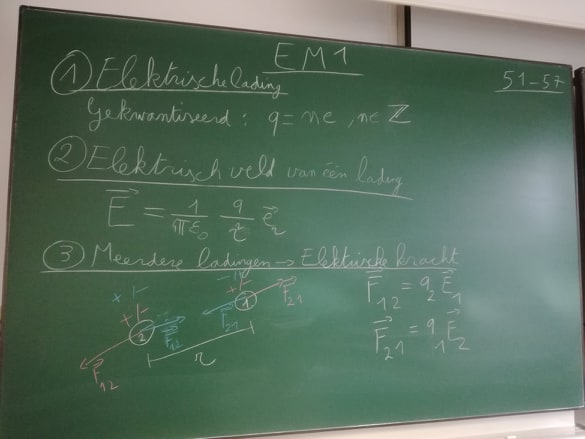
\includegraphics[width=0.9\textwidth]{Bord1a}
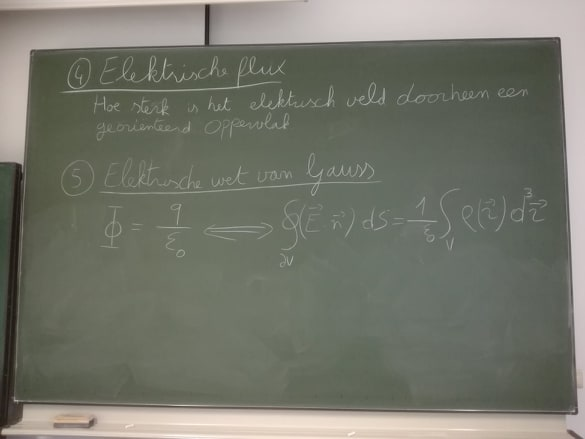
\includegraphics[width=0.9\textwidth]{Bord1b}
\end{center}
\newpage

\subsection*{Bijlage 1.2: opgeloste oefeningen}



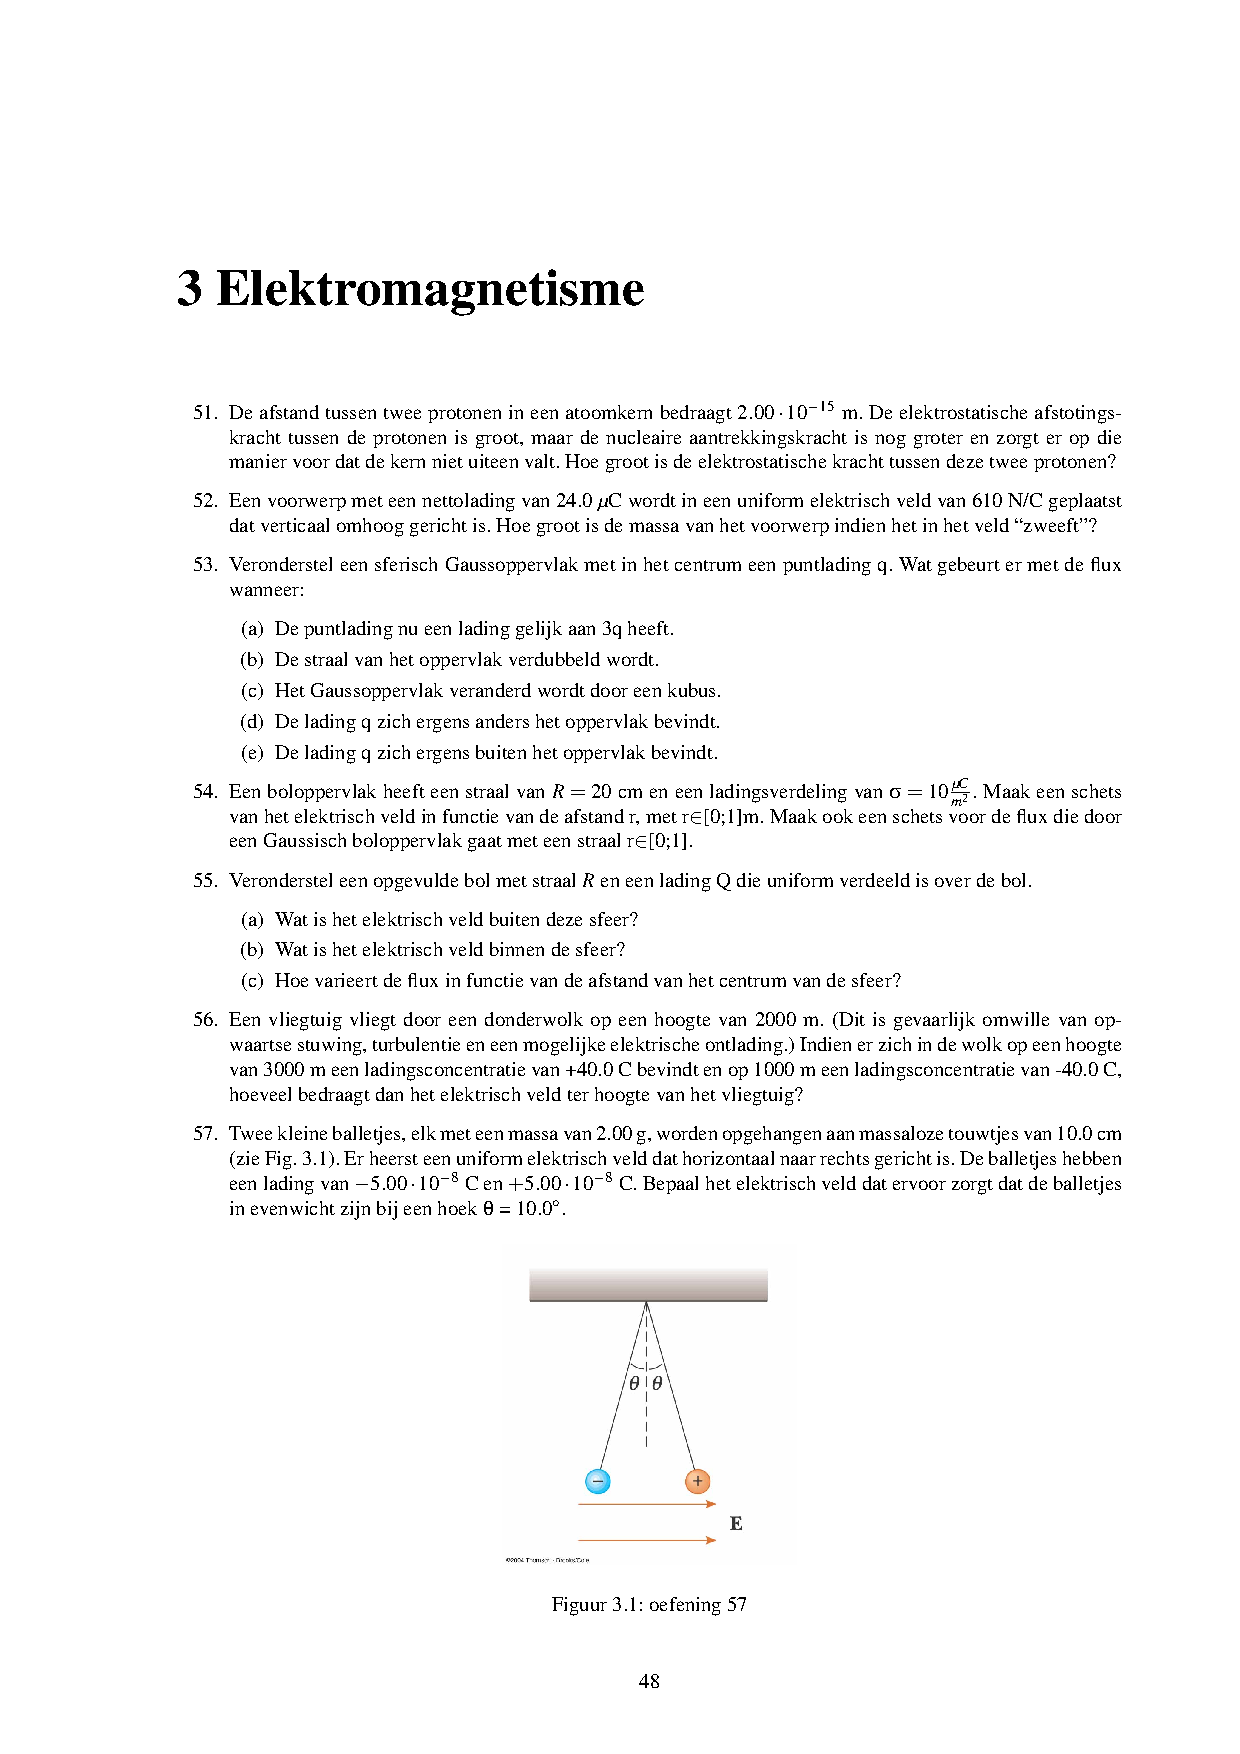
\includepdf[scale = 0.95,pages = 1,pagecommand=\subsection*{Bijlage 1.3: oefeningenbundel elektromagnetisme}]{OefeningenBundel}
\includepdf[scale = 0.95,pages =2-,pagecommand=]{OefeningenBundel}